%% ============================================================
%%  04_umsetzung.tex
%%  Kapitel 4: Umsetzung / Implementierung
%% ============================================================
\chapter{Umsetzung und Implementierung der Abstraktionsschicht}
\label{chap:umsetzung}

In diesem Kapitel wird aufgezeigt, wie die Abstraktionsschicht aufgebaut und in den Executor integriert wurde. Hierbei wird zudem besprochen, welche Objekte zur Umwandlung genutzt wurden und weshalb.

\section{Ausgangslage}
\label{sec:ausgangslage}

Vor der Integration einer Definitionsschicht der Circuits gab es bereits die Basis der API-Anbindungen. Der damalige Ansatz bestand darin, einen Schaltkreis über \textit{Qiskit}-Objekte zu definieren und anschließend an das Backend zu übergeben. Damit nutzte man jedoch keinen backendunabhängigen Ansatz, sondern lediglich einen Wrapper um \textit{Qiskit}-Objekte. Jeder Schaltkreis war intern ein \texttt{qiskit.QuantumCircuit}, jede Observable eine \texttt{qiskit.SparsePauliOp} und jeder Parameter ein \textit{Qiskit}-\texttt{ParameterVector} oder dessen Element. Wollte man ein anderes Backend als \textit{Qiskit} verwenden, mussten diese \textit{Qiskit}-Objekte zunächst in das jeweilige Backend-Format zurückübersetzt werden. Dadurch war das Programm ineffizient und von \textit{Qiskit} abhängig.

\section{Wahl der internen Objekte}
\label{sec:interne-objekte}

Zunächst musste entschieden werden, in welches Format die Abstraktion die frameworkunabhängigen Objekte später umwandelt.
Bei der Wahl der internen Objekte in \textit{PennyLane} gab es zwei Optionen. In \textit{PennyLane} unterscheidet man zwischen den Objekten \enquote{Quantum Tape} und \enquote{Quantum Node}, um Circuits als Objekt zu erstellen.

Das Quantum Tape ist die unterste Abstraktionsschicht und wird hauptsächlich für die Entwicklung von Erweiterungen für \textit{PennyLane} genutzt, da es einen kleineren Overhead hat. Das Tape zeichnet die angewendeten Gatter als Liste von Operationen auf. Die Parameter der Gatter werden dabei als \textit{PennyLane}-NumPy-Arrays gespeichert. Dies ist ein Wrapper der \textit{NumPy}-Bibliothek, der die Parameter als differenzierbar markiert. Dadurch wird Backpropagation durch den Circuit möglich.
Der Quantum Node ist eine Abstraktion des Quantum Tapes und die übliche Weise, einen Circuit zu erstellen. Dieses Objekt lässt sich durch den Python-Decorator \texttt{@qml.qnode} erstellen. Intern wird beim Aufruf des QNodes ein Tape erstellt und anschließend auf dem Device ausgeführt. Im Gegensatz zum Tape bietet der QNode mehrere Konfigurationsmöglichkeiten. Eine der wichtigsten hierbei ist die Option \texttt{diff\_method="best"}, um eine alternative Differenzierungsmethode zu Parameter-Shift nutzen zu können. Funktional spricht dies für den QNode, hinsichtlich der Laufzeit war jedoch ein Vorteil der Tapes zu erwarten.

Um die beiden Objekte gegenüberzustellen, wurden zwei Vergleichsebenen
betrachtet. Auf der ersten Ebene wurden Tape und QNode mit derselben
Differenzierungsmethode (Parameter-Shift) betrieben. Damit lässt sich der
reine Overhead isolieren, der durch die zusätzliche Abstraktionsschicht des QNodes entsteht, unabhängig davon, wie der Gradient berechnet wird. Auf
der zweiten Ebene wurde der QNode zusätzlich mit der Option
\texttt{diff\_method="best"} gemessen. In diesem Modus wählt
\textit{PennyLane} auf dem Simulator \texttt{default.qubit} automatisch
Backpropagation, die im Gegensatz zur Parameter-Shift-Regel nicht linear
mit der Anzahl trainierbarer Parameter skaliert~\cite{mitarai2018,schuld2019}.
Dieser Messpunkt bildet damit den Vorteil ab, den der QNode im
praktischen Einsatz bietet, nämlich den Zugriff auf effizientere
Differenzierungsmethoden ohne manuelle Implementierung der zugehörigen
Ausführungslogik.

Die Messungen wurden für Circuits mit 5, 8, 10 und 12 Qubits durchgeführt
und decken jeweils die Phasen Circuit-Erstellung, Ausführung und
Gradientenberechnung bei 10\,000 Gattern und 4 Iterationen ab. Bei der
Gradientenberechnung besitzen 30\,\% der Gatter trainierbare Parameter, die
über den Schaltkreis verteilt wurden. Die Ergebnisse sind in
Abbildung~\ref{fig:alle_time} dargestellt.

\begin{figure}[H]
    \centering
    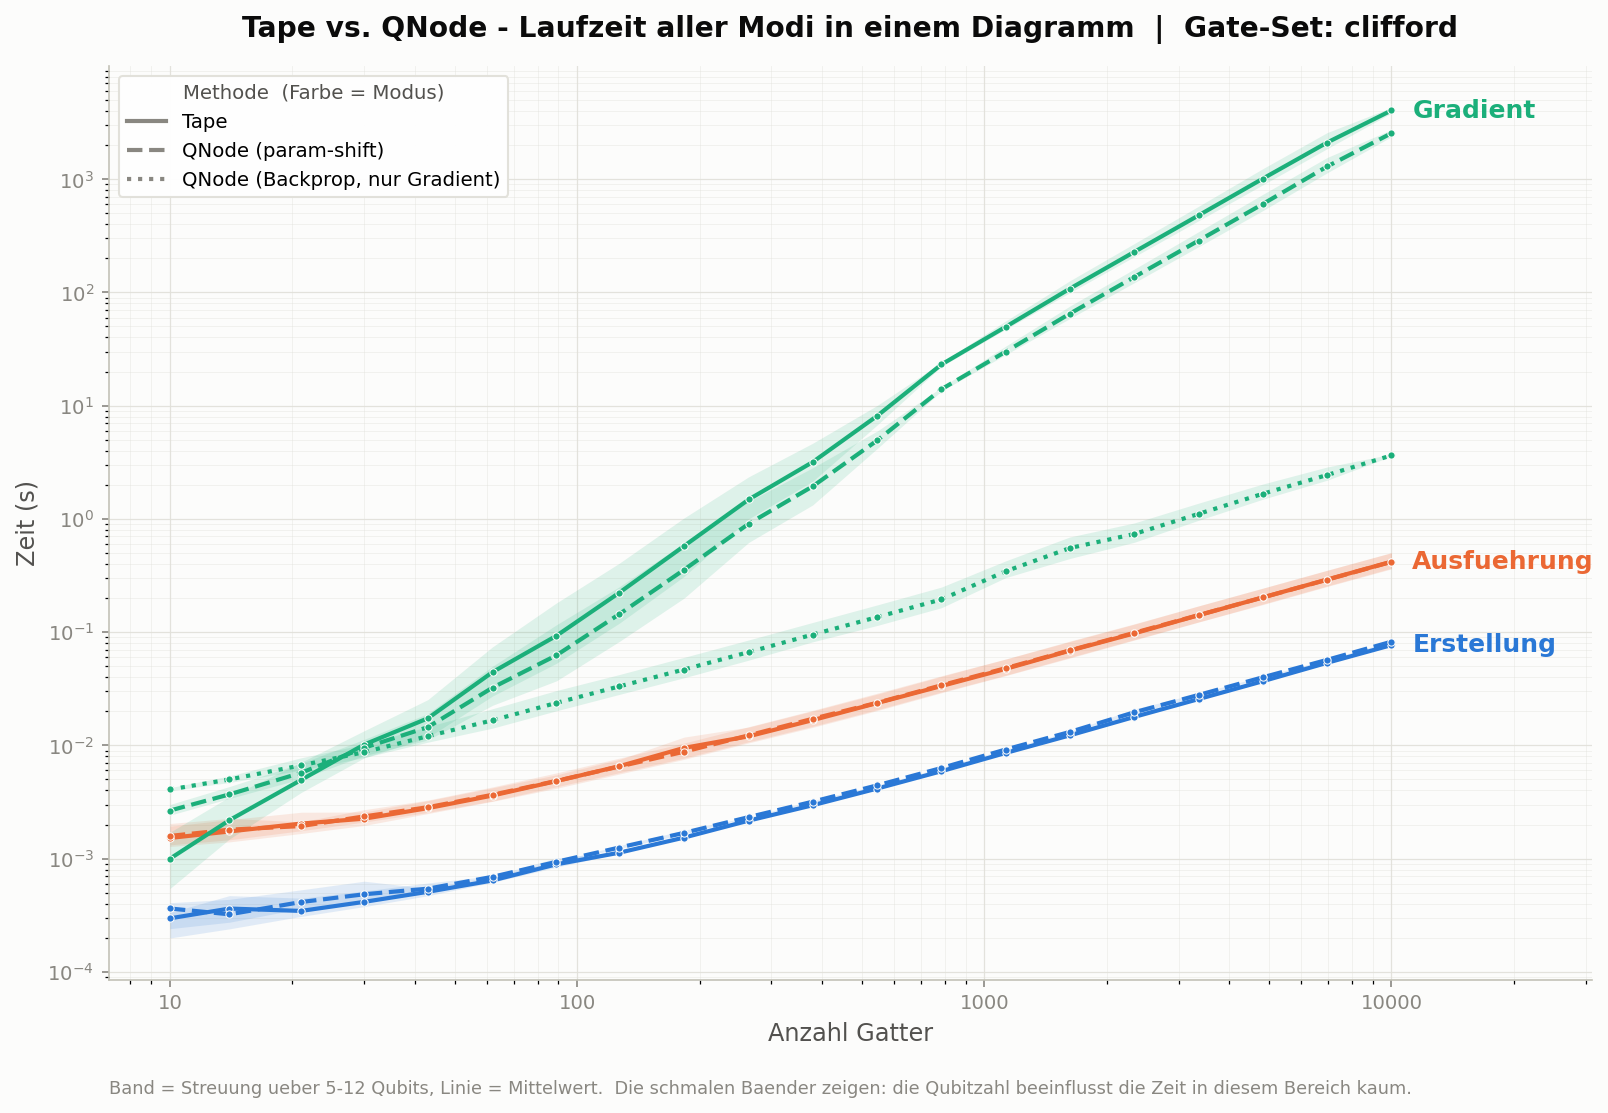
\includegraphics[width=1.0\textwidth]{figures/QnodevsTape/alle_modi_ein_diagramm_time.png}
    \caption{Laufzeiten von Tape und QNode für Erstellung,
  Ausführung und Gradientenberechnung als Mittelwert von 5, 8, 10 und 12 Qubits}
    \label{fig:alle_time}
\end{figure}

Es lässt sich erkennen, dass sowohl bei der Erstellung als auch bei der Ausführung und der Gradientenberechnung mittels Parameter-Shift kaum ein Unterschied zwischen den Tapes und den QNodes besteht. Zudem zeigt sich, dass die QNodes bei der Gradientenberechnung mit
Backpropagation bei 10\,000 Gattern einen Geschwindigkeitsvorteil von rund
36\,\% bis 38\,\% gegenüber den rohen Tapes haben. Parameter-Shift ist allgemein
deutlich langsamer als die \textit{best}-Methode (Backpropagation), da Parameter-Shift zwei
Schaltkreis-Auswertungen pro trainierbarem Parameter benötigt (bei einer Anzahl von 3000 trainierbaren Gattern also $\approx 2 \cdot 3000 = 6000$
Auswertungen), während Backpropagation den vollständigen Gradienten in einem
einzigen Vor- und Rückwärtslauf unabhängig von der Parameterzahl berechnet.
Damit skaliert Parameter-Shift näherungsweise mit
$\mathcal{O}(\text{Gatter}^2)$, Backpropagation dagegen mit
$\mathcal{O}(\text{Gatter})$.

Ein weiteres wichtiges Argument für den QNode war, dass die Parameter der Gatter im Tape nur als feste Werte vorliegen und sich nicht als mathematische Ausdrücke angeben lassen. Da der QNode über eine Python-Funktion definiert wird, gehen die Parameter dort als Argumente ein und können in mathematischen Ausdrücken verwendet werden, bevor sie auf die Gatter angewendet werden. Das passende Tape entsteht daraus erst mit konkreten Werten.

Anders als in \textit{PennyLane} gibt es in \textit{Qiskit} nur ein Circuit-Objekt, den \texttt{QuantumCircuit}. Dieser entspricht dem Tape und war damit die einzige Wahl als internes Zielformat. Ein Gegenstück zum QNode gibt es nicht. Die Gradienten werden stattdessen über separate Parameter-Shift-Klassen aus \texttt{qiskit\_algorithms.gradients} berechnet~\cite{schuld2019}.
\newpage
\section{Implementierung der Abstraktion}
\label{sec:implementierung-abstraktion}

\begin{figure}[H]
    \centering
    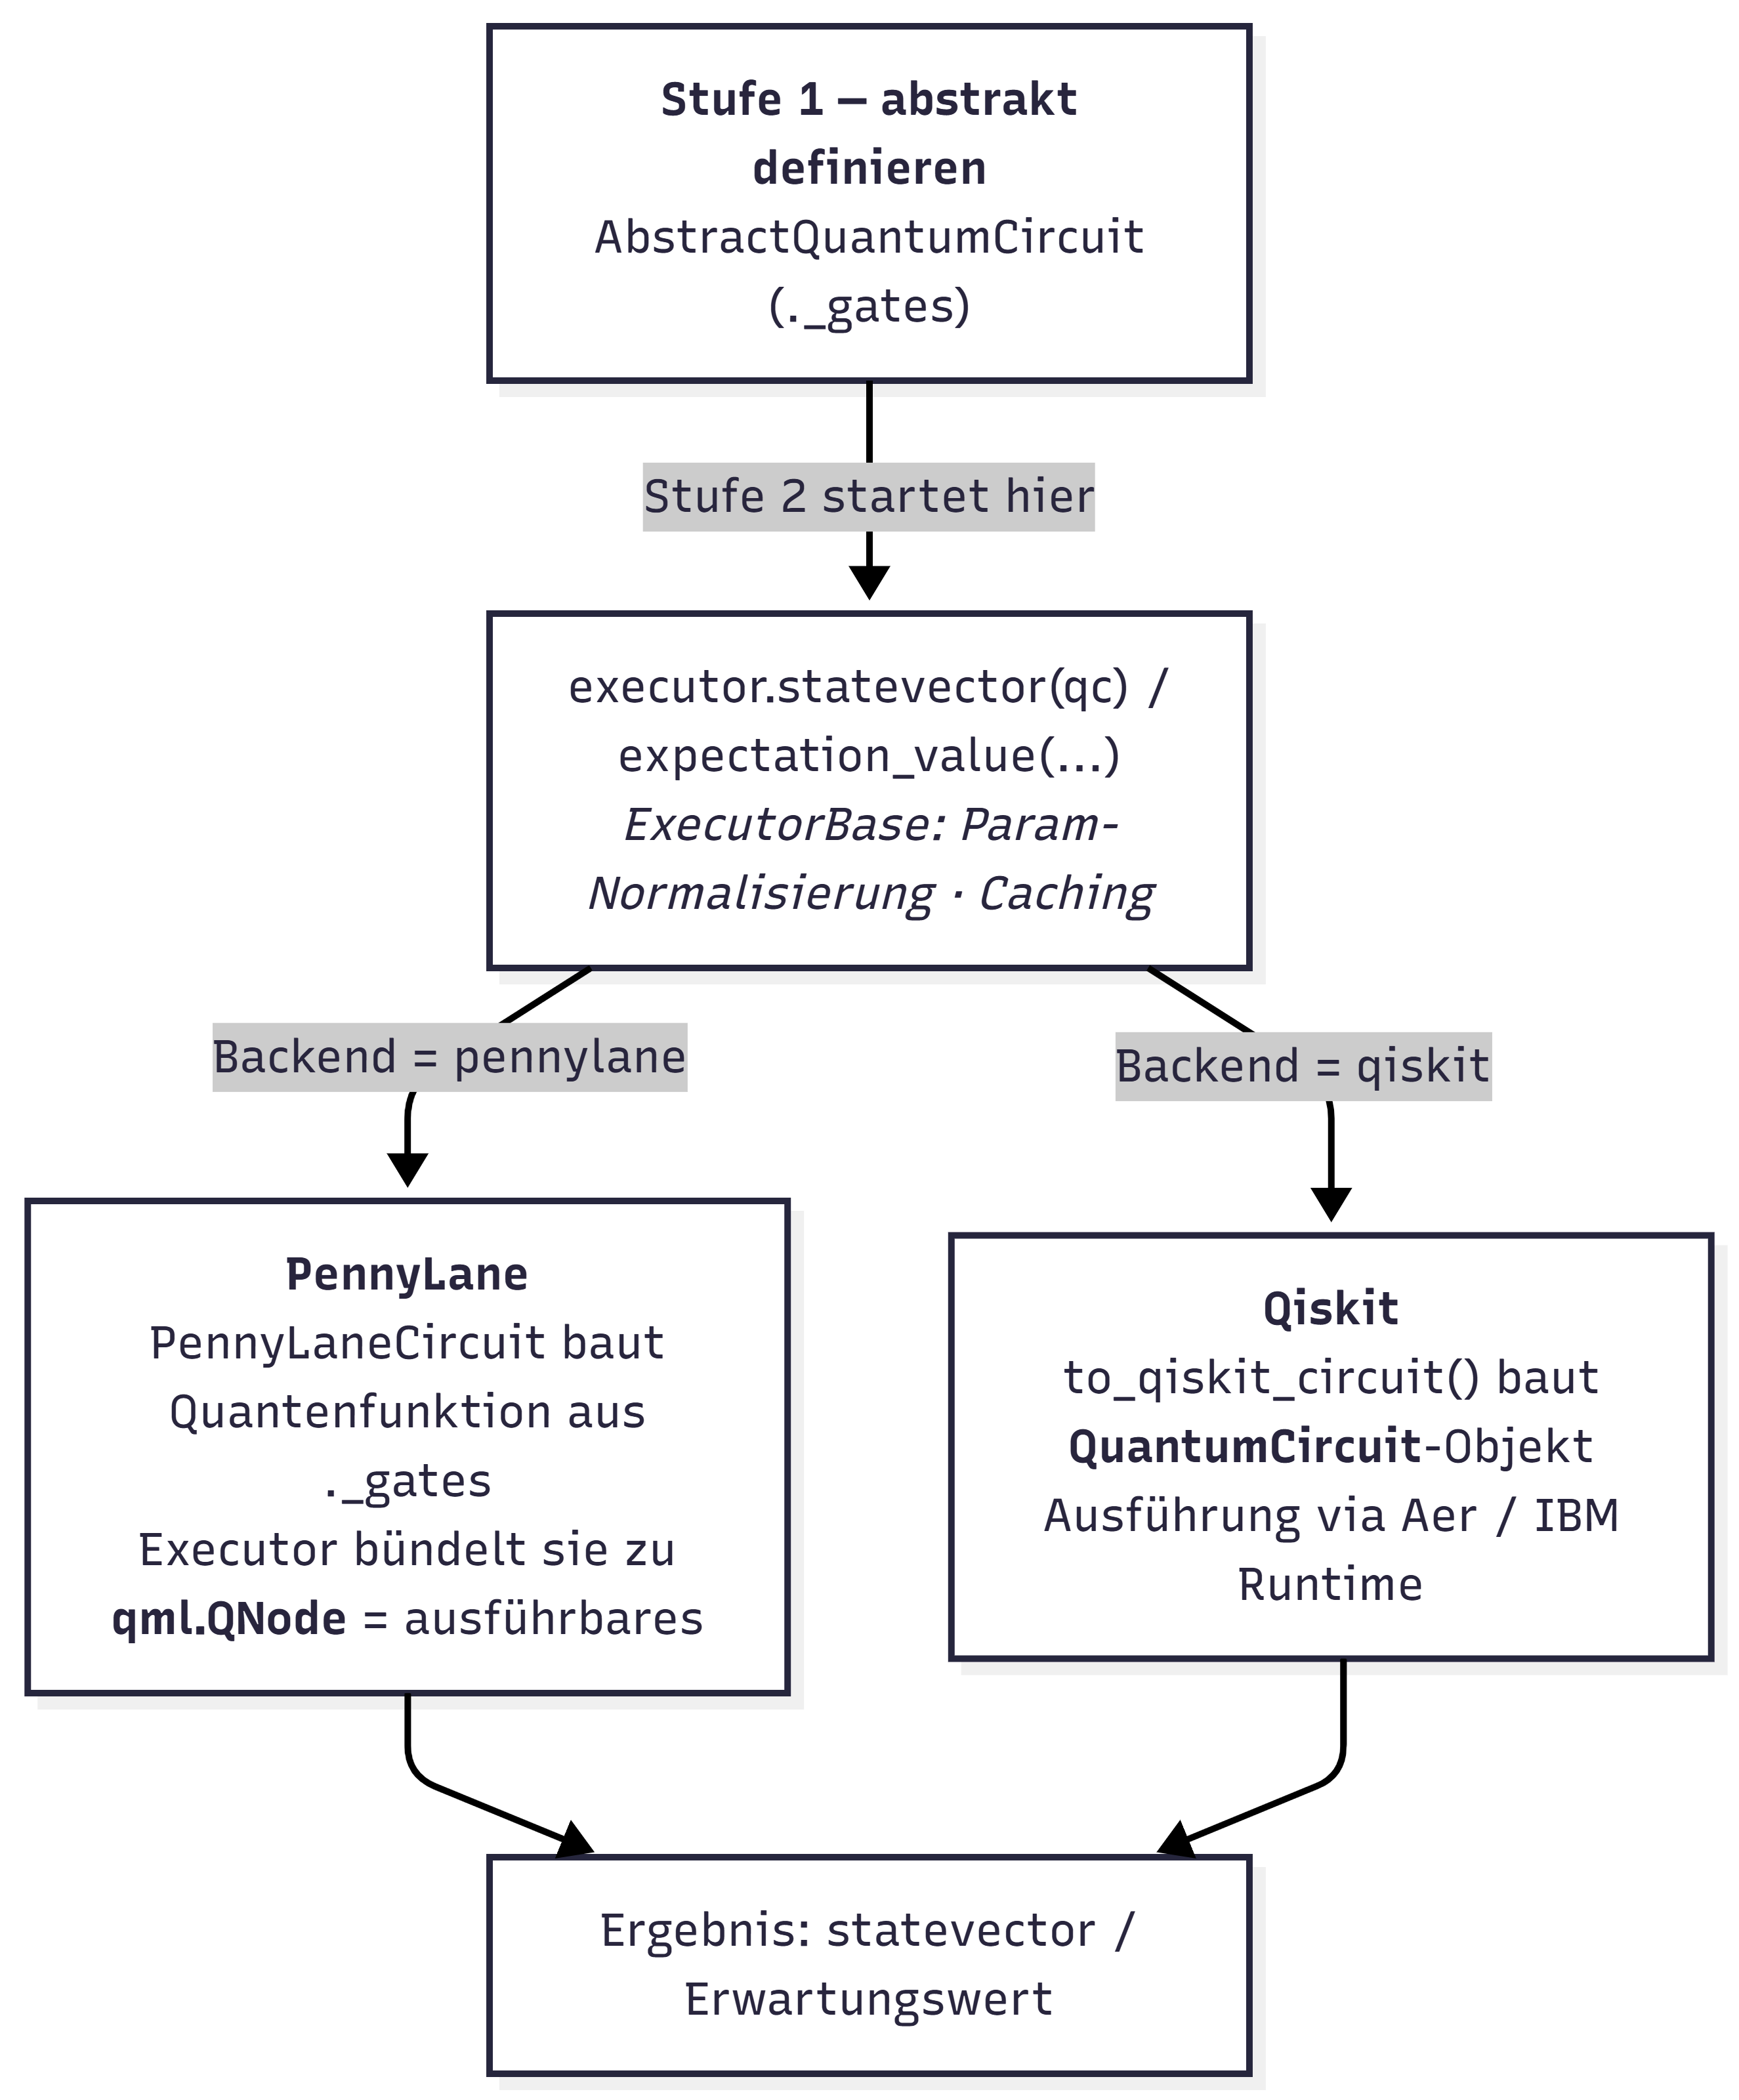
\includegraphics[width=0.6\textwidth]{figures/abstraction-architektur.png}
    \caption{Architektur der Abstraktion}
    \label{fig:abstraktion_architektur}
\end{figure}

Grundlage der Abstraktionsschicht ist eine Datenstruktur, mit der sich ein
Schaltkreis und Observablen über eine eigene, vom Framework unabhängige Syntax beschreiben
lassen. Die wesentliche Schwierigkeit bestand darin, den gemeinsamen
Funktionsumfang der unterstützten Frameworks zu ermitteln, da nur solche
Konstrukte in die Abstraktion aufgenommen werden können, die sich in jedem
Ziel-Backend nachbilden lassen.

Die Abstraktionsschicht ruht auf vier Datentypen, aus denen jedes Backend
anschließend seine eigenen, nativen Objekte erzeugt. Entscheidend ist, dass
diese vier Typen frameworkunabhängig sind. Sie beschreiben, \textit{was}
ausgeführt und gemessen werden soll, treffen jedoch keinerlei Annahmen über das
ausführende Framework und importieren insbesondere keines davon. Damit wird die
im Konzept geforderte Trennung von Definition und Ausführung
(Abschnitt~\ref{sec:konzept-loesung}) auf der Ebene der Datentypen konkret. Die
Nutzerinnen und Nutzer definieren ihren Schaltkreis einmalig in dieser abstrakten Form, während die Übersetzung in ein konkretes Framework erst später und lokal im jeweiligen Backend erfolgt. Hierbei lässt sich das Framework durch das Ändern einer einzigen Variablen wechseln.

\paragraph*{Der Schaltkreis}\mbox{}\\
\label{par:datentypen-schaltkreis}
Ein Schaltkreis wird framework-unabhängig als geordnete Liste typisierter
Gate-Objekte gehalten. Die Reihenfolge der Listenelemente bestimmt die
Ausführungsreihenfolge. Aus dieser Repräsentation ergeben sich zwei
Eigenschaften. Zum einen stellen alle Schaltkreis-Operationen wie das Verketten,
Invertieren, Kopieren und das Binden von Parametern Umformungen dieser Liste dar
und erfordern keinen Aufruf einer Framework-Funktion. Zum anderen gelangt jedes
Gatter über eine einzige Stelle in die Liste, an der die Validierung erfolgt.
Geprüft werden die Zugehörigkeit zum gemeinsamen Vokabular, die erwartete Form
des Gatters hinsichtlich der Zahl seiner Qubits und Winkel sowie die Einhaltung
der Registergröße. Nicht unterstützte Konstrukte werden dadurch bereits bei der
Definition zurückgewiesen und nicht erst beim Aufbau des nativen Schaltkreises,
bei dem sich der Ort der Fehlermeldung deutlich von der Ursache entfernen würde.

\paragraph*{Das Gate-Vokabular}\mbox{}\\
\label{par:datentypen-vokabular}
Ein einzelnes Gatter wird framework-unabhängig als \textit{Dataclass}
abgebildet. Die Abstraktion unterscheidet dabei lediglich zwei Formen, ein
\texttt{CliffordGate} für parameterfreie Gatter wie \texttt{h} oder \texttt{cx}
und ein \texttt{RotationGate} für einwinklige Gatter wie \texttt{rx} oder
\texttt{rzz}. Die Beschränkung auf zwei Formen folgt aus der Anforderung, dass jedes
Backend das Gatter ohne vorherige Zerlegung abbilden können muss.

Die zulässigen Gatternamen werden ausschließlich durch die Registry
\texttt{SUPPORTED\_GATES} festgelegt, die in der umgesetzten Fassung 33 Gatter
umfasst. Sie dient als einzige verbindliche Referenz, aus der sowohl die
Validierung als auch die Übersetzer beider Backends lesen. Ein Eintrag ist erst
dann gültig, wenn er an drei Stellen zugleich verfügbar ist, und zwar als
Methode auf \textit{Qiskit}s \texttt{QuantumCircuit}, als Schlüssel im
Übersetzungswörterbuch des \textit{PennyLane}-Backends sowie, sofern das Gatter
parameterfrei ist, in den Inversionstabellen der Abstraktion. Rotationen werden
stattdessen über das Vorzeichen ihres Winkels invertiert.

Da die Konsistenz dieser drei Stellen technisch nicht erzwungen wird, sichert
ein eigener Paritätstest sie ab. Dieser beschränkt sich nicht auf die Prüfung
der Existenz, sondern vergleicht die von beiden Backends erzeugten
Unitärmatrizen und verifiziert, dass Gatter und Inverses gemeinsam die Identität
ergeben. Ein neu aufgenommenes Gatter ohne angebundenes Backend führt daher zu
einem Fehlschlag der Testsuite und nicht zu einem Fehler zur Laufzeit.

\paragraph*{Die Observable}\mbox{}\\
\label{par:datentypen-observable}
Das Gegenstück zum Schaltkreis beschreibt die zu messende Größe, also das
\texttt{observable}-Argument von \texttt{expectation\_value}. Dieses akzeptiert
wahlweise eine einzelne Observable oder eine Liste davon, sodass mehrere
Erwartungswerte in einem Aufruf ausgewertet werden können. Die Speicherung
erfolgt ebenfalls rein datenbasiert als Liste von Pauli-Strings mit zugehörigen
Koeffizienten. Beispielsweise beschreibt \verb|["ZZ", "IX"]| mit \verb|[0.5, 0.3]| den Operator $0{,}5\,Z_0Z_1 + 0{,}3\,X_0$. Da die Observable
framework-unabhängig bleibt, umfasst die Komponente eine eigene Pauli-Algebra.
Die Verknüpfung zweier Operatoren sowie das Zusammenfassen gleichartiger Terme
sind auf Basis einer Produkttabelle der einzelnen Pauli-Zeichen eigenständig
implementiert. Festgelegt ist zudem eine Little-Endian-Konvention, bei der das
rechte Zeichen Qubit\,0 bezeichnet. Eine derartige Festlegung ist einmalig zu treffen und anschließend
in jedem Übersetzer zu berücksichtigen. \textit{PennyLane} ordnet Pauli-Zeichen
dagegen von links nach rechts zu, was als Big-Endian bezeichnet wird, weshalb das
entsprechende Backend das Label vor der Übergabe umkehrt. Bei der Umwandlung für
das \textit{Qiskit}-Backend ist dies nicht nötig, da \textit{Qiskit} bereits
Little-Endian nutzt.

\paragraph*{Die Parameter}\mbox{}\\
\label{par:parameter}
Ein Parameter stellt einen symbolischen Platzhalter für einen Zahlenwert dar und
ist als Unterklasse von \texttt{sympy.Symbol} realisiert. Jeder Parameter trägt
den Namen seines Vektors sowie einen Index und wird als \texttt{theta[0]}
notiert. Die Symbole werden zudem auf die reelle Domäne eingeschränkt, was der
projektweiten Annahme ausschließlich reeller Parameter entspricht.

Aus dieser Realisierung ergeben sich zwei Eigenschaften. Erstens sind Parameter
vollwertige \textit{SymPy}-Symbole, sodass ein Ausdruck wie \texttt{2*theta[0] +
theta[1]} unmittelbar gültig ist, ohne dass eine eigene Arithmetik oder ein
eigener Ausdrucksbaum implementiert werden müsste. Die symbolische Auswertung
übernimmt \textit{SymPy}. Zweitens enthält ein solcher Ausdruck ausschließlich Daten und
keinerlei Framework-Bezug. Derselbe Ausdruck kann daher an beiden Stellen
verwendet werden, an denen die Abstraktion einen Zahlenwert erwartet, nämlich
als Gate-Winkel und als Operator-Koeffizient.

Der \texttt{ParameterVector} fasst Parameter zu einer benannten, indexierten und
in ihrer Länge veränderbaren Folge zusammen. Die in einem Schaltkreis oder
Operator enthaltenen Parameter werden stets nach Vektorname und Index sortiert
zurückgegeben. Diese deterministische Ordnung ist keine bloße Formalie, sondern
definiert die Reihenfolge, in der die Backends die Parameterwerte zur
Ausführungszeit erwarten.

Die Übersetzung in den Parametertyp des jeweiligen Frameworks übernimmt das
Backend. In beiden Fällen wird hierfür \textit{SymPy}s \texttt{lambdify} eingesetzt,
allerdings zu unterschiedlichen Zwecken. Für \textit{Qiskit} wird der Ausdruck auf die
Elemente eines \textit{Qiskit}-\texttt{ParameterVector} angewandt und dadurch als
\textit{Qiskit}-\texttt{ParameterExpression} rekonstruiert, bleibt also symbolisch. Für
\textit{PennyLane} wird der Ausdruck hingegen in eine numerisch auswertbare Funktion
überführt, die zur Ausführungszeit mit den konkreten Parameterwerten aufgerufen
wird. Ein und derselbe Mechanismus bedient somit sowohl die symbolische als auch
die numerische Zielrepräsentation.

\section{Integration in den Executor}
\label{sec:integration}

Die Abstraktion beschreibt bisher nur die Definition eines Schaltkreises und einer
Observable. Ausgeführt wird beides über den bereits vorhandenen Executor, weshalb die
Abstraktion an drei Stellen in die bestehende Basis eingefügt werden musste, und zwar in die
Basisklassen, in die Backends und in die Auswahl des Backends.

Die Basisklassen \texttt{QuantumCircuitBase} und \texttt{QuantumOperatorBase} legen fest,
welche Methoden ein Schaltkreis und eine Observable bereitstellen müssen. Bisher waren sie
auf \textit{Qiskit} typisiert, da ihre Winkel und Parameter als \textit{Qiskit}-Objekte
angegeben waren. Diese Angaben wurden entfernt. Ob ein Winkel umgerechnet oder unverändert
an das Gatter durchgereicht wird, entscheidet sich nun daran, ob es sich um eine Zahl
handelt, und nicht mehr am Typ des Objekts. Dadurch arbeiten die zusammengesetzten Methoden
der Basisklasse wie \texttt{pauli\_evolution} mit den symbolischen Parametern der
Abstraktion genauso wie zuvor mit denen von \textit{Qiskit}. Die Abstraktion erbt selbst von
diesen Basisklassen und ist damit kein zusätzliches Format neben dem bestehenden, sondern
dessen Umsetzung.

Die Übersetzung in das native Format geschieht erst im Backend. Jedes Backend besitzt dafür
einen Eintrittspunkt, der aus dem abstrakten Objekt das native erzeugt. Entscheidend ist
dabei weniger, was dieser annimmt, als was er ablehnt. Übergeben werden dürfen nur Objekte
der Abstraktion, ein \texttt{qiskit.QuantumCircuit} wird zurückgewiesen. Damit ist der
eingangs beschriebene Weg über \textit{Qiskit}-Objekte geschlossen, diese sind nur noch das
Ergebnis der Übersetzung und nicht mehr deren Eingabe. Blieben beide Wege offen, bestünde die
Abhängigkeit von \textit{Qiskit} weiterhin. Aus demselben Grund prüft auch das
\textit{Qiskit}-Backend jeden Gatternamen gegen \texttt{SUPPORTED\_GATES}, obwohl
\textit{Qiskit} das Gatter selbst auflösen könnte. Andernfalls ließen sich Schaltkreise
definieren, die nur auf \textit{Qiskit} lauffähig sind. Das Ergebnis der Übersetzung wird
über den Hash des abstrakten Objekts zwischengespeichert und nur nach einer Änderung neu
erzeugt.

Am Executor selbst waren nur wenige Ergänzungen nötig. Eine übergebene Observable wird vor
der Ausführung selbsttätig in den nativen Typ gewandelt, sodass die Abstraktion direkt an
\texttt{expectation\_value} übergeben werden kann. Die Parameterwerte werden weiterhin über
den Namen des Vektors angegeben, etwa \texttt{theta=[0.3, 0.7]}. Welcher Wert bei welchem
Symbol landet, entscheidet die weiter oben beschriebene Sortierung nach
Vektorname und Index, an der sich beide Backends beim Binden orientieren. Eine falsche
Zuordnung würde keinen Fehler auslösen, sondern lediglich ein falsches Ergebnis liefern.

Welches Backend verwendet wird, entscheidet die Factory über \texttt{Executor.create()}. Sie
hält eine Registry aus Backend-Namen und den zugehörigen Klassen, in die sich ein Backend
beim Import selbst einträgt. Die Definition von Schaltkreis und Observable bleibt beim
Wechsel unverändert, geändert wird allein der Name des Backends.

Zuletzt wurden die alten Wrapper entfernt, in denen Schaltkreis, Observable und Parameter als
\textit{Qiskit}-Objekte gehalten wurden. Dadurch importieren weder die Basisklassen noch die
Abstraktion noch das \textit{PennyLane}-Backend \textit{Qiskit}. Die Installation des
\textit{PennyLane}-Backends zieht \textit{Qiskit} nicht mehr nach, was zuvor nicht möglich
war, da die Übersetzung nach \textit{PennyLane} über \textit{Qiskit}-Objekte lief.

\chapter{Vorteile der Abstraktionsschicht}
\label{chap:vorteile}

Die in Kapitel~\ref{chap:umsetzung} beschriebene Abstraktionsschicht adressiert
vier wiederkehrende Probleme bei der Arbeit mit mehreren
Quantencomputing-Frameworks. Dazu zählen die Bindung des Programmcodes an eine
konkrete Framework-Syntax, die eingeschränkte Vergleichbarkeit von
Implementierungen, der Installationsaufwand paralleler Framework-Stacks und die
Instabilität der Framework-APIs über Versionsgrenzen hinweg. Die folgenden
Abschnitte behandeln diese Punkte einzeln. Abschnitt~\ref{sec:vorteile_grenzen}
grenzt anschließend ab, welche Zusagen die Abstraktion nicht macht.

\section{Einheitliche Definitionsschnittstelle}
\label{sec:vorteile_einheitlich}

Der zentrale Effekt der Abstraktion besteht darin, dass für die Beschreibung
eines Schaltkreises und einer Observablen genau ein Weg existiert. Ein
Schaltkreis wird ausschließlich über \texttt{AbstractQuantumCircuit} definiert,
eine Observable ausschließlich über \texttt{AbstractQuantumOperator}. Welche
Gatter zulässig sind, ergibt sich aus einem einzigen, explizit gepflegten
Vokabular in \texttt{SUPPORTED\_GATES}. Jedes hinzugefügte Gatter wird
unmittelbar dagegen validiert.

Ein Wechsel des Ausführungsbackends erfordert dadurch keine Änderung der
Problembeschreibung. Ein direkt gegen ein Framework geschriebenes Programm muss
bei einem Wechsel vollständig auf die Syntax und die Objektmodelle des
Zielframeworks portiert werden. Hier beschränkt sich der Eingriff auf den
Austausch der Executor-Instanz.

\begin{lstlisting}[language=Python]
# Schaltkreisdefinition, backendunabhängig
qc = AbstractQuantumCircuit(2)
qc.h(0)
qc.cx(0, 1)
# Auswahl des Backends
executor = Executor.create("qiskit")
# executor = Executor.create("pennylane")
\end{lstlisting}

Neben der Ersparnis an Portierungsaufwand ist vor allem die methodische
Konsequenz relevant. Da beide Ausführungen aus derselben Schaltkreisdefinition
hervorgehen, ist die Formulierung des Problems über alle Backends hinweg eine
kontrollierte Größe. Beobachtete Unterschiede in Laufzeit oder Ergebnis lassen
sich damit auf das Backend zurückführen und nicht auf eine abweichende
Formulierung des Schaltkreises. Diese Eigenschaft ist die Voraussetzung für die
in Kapitel~\ref{chap:evaluation} durchgeführten Vergleichsmessungen. Ohne sie
wäre ein Backend-Vergleich stets mit dem Implementierungsstil der jeweiligen
Referenzimplementierung vermischt.

Die zentrale Validierung verlagert Fehler zudem nach vorn. Ein unbekannter
Gatter-Name oder eine falsche Qubit-Anzahl führt bereits beim Aufbau des
Schaltkreises zu einer Ausnahme. Andernfalls würde der Fehler erst bei der
Ausführung im Backend auftreten und dort nur in framework-spezifischer
Terminologie sichtbar.

\section{Modularisierbarkeit}
\label{sec:vorteile_modular}

Die Abstraktion zerlegt ein Quantenprogramm in austauschbare Bestandteile. Dies
betrifft sowohl die Trennung von Definition und Ausführung als auch den Aufbau
eines Schaltkreises aus einzelnen Teilen.

\paragraph*{Trennung von Definition und Ausführung}\mbox{}\\
Die Beschreibung des Problems ist vollständig von seiner Ausführung getrennt.
Das Paket \texttt{abstraction} enthält keinerlei Framework-Importe. Die
Übersetzung in ein natives Format findet erst zur Laufzeit innerhalb des
jeweiligen Backends statt. Der Nutzercode hängt damit von den abstrakten
Verträgen in \texttt{base} ab und nicht von einer konkreten Implementierung. Dies
entspricht dem Dependency-Inversion-Prinzip~\cite{martin2003agile}. Ein Programm
ist dadurch kein \enquote{\textit{Qiskit}-Programm} oder
\enquote{\textit{PennyLane}-Programm} mehr, sondern ein Programm, das auf
\textit{Qiskit} oder \textit{PennyLane} ausgeführt wird. Die Methode
\texttt{switch\_backend} überträgt zusätzlich die bestehende Konfiguration auf
ein anderes Backend.

\paragraph*{Zusammensetzen von Teilschaltkreisen}\mbox{}\\
Ein Schaltkreis liegt intern als typisierte Liste von Gatter-Objekten vor und
nicht als framework-spezifische Datenstruktur. Er lässt sich dadurch wie ein
wiederverwendbarer Baustein behandeln. \texttt{compose} setzt einen
Teilschaltkreis an einer frei wählbaren Qubit-Position ein und macht ihn damit
ortsunabhängig. \texttt{invert} erzeugt das zugehörige Gegenstück und
\texttt{copy} stellt sicher, dass sich mehrfach verwendete Bausteine nicht
gegenseitig beeinflussen. Variationsalgorithmen lassen sich so in getrennt
entwickelbare und einzeln testbare Blöcke gliedern, etwa in Zustandspräparation,
Ansatz und Basiswechsel.

\paragraph*{Späte Parameterbindung}\mbox{}\\
Symbolische Parameter beschreiben einen Schaltkreis, dessen Zahlenwerte noch
offen sind. Sie werden erst bei der Ausführung übergeben, sodass derselbe
Schaltkreis mit beliebig vielen Parametersätzen wiederverwendet werden kann. Für
einen klassischen Optimierer genügt damit der Zugriff auf die Parameter und den
zugehörigen Erwartungswert. Der innere Aufbau des Schaltkreises bleibt ihm
verborgen, wodurch sich Optimierung und Schaltkreisdefinition unabhängig
voneinander entwickeln lassen.

\paragraph*{Erweiterbarkeit}\mbox{}\\
Die Backends sind der Abstraktion nicht namentlich bekannt. Sie registrieren sich
über eine Registry und werden zusätzlich über Entry-Points der Gruppe
\texttt{qc\_executor.backends} entdeckt. Ein zusätzliches Backend erweitert das
System, ohne dass Änderungen am Kern erforderlich sind. Dies entspricht dem
Open-Closed-Prinzip.

\section{Optionale Framework-Abhängigkeiten}
\label{sec:vorteile_abhaengigkeiten}

Da die Abstraktion selbst kein Framework importiert, muss auch nicht die
Gesamtheit der unterstützten Frameworks installiert sein. Die Backends sind als
optionale Installationsvarianten deklariert und werden beim Import in einem
\texttt{try}/\texttt{except~ImportError}-Block geladen. Ein nicht installiertes
Framework deaktiviert ausschließlich das zugehörige Backend, während alle
übrigen Backends unverändert nutzbar bleiben. Der Versuch, ein nicht verfügbares
Backend zu erzeugen, führt zu einer Fehlermeldung mit dem passenden
Installationshinweis.

Praktisch ist dies aus zwei Gründen relevant. Zum einen reduziert es den Umfang
einer Installation auf die tatsächlich benötigten Komponenten, was insbesondere
in Container- und CI-Umgebungen ins Gewicht fällt. Zum anderen entschärft es
Abhängigkeitskonflikte. Die unterstützten Frameworks geben teilweise eigene und
gegenseitig unverträgliche Versionsbereiche für gemeinsame Basisbibliotheken vor.
Da sich nur eine Teilmenge der Backends installieren lässt, addieren sich diese
Einschränkungen nicht zu einem unauflösbaren Gesamtsystem.

\newpage
\section{Entkopplung von Framework-Versionen}
\label{sec:vorteile_versionen}

Die APIs der betrachteten Frameworks unterliegen einer erheblichen Änderungsrate.
Hauptversionswechsel gehen regelmäßig mit dem Entfernen oder Umbenennen
öffentlicher Schnittstellen einher. Ohne Abstraktionsschicht wirkt sich eine
solche Änderung unmittelbar auf jedes Anwendungsprogramm aus, das die betroffene
Schnittstelle verwendet.

Die Abstraktion begrenzt die Reichweite derartiger Änderungen strukturell. Da
Framework-Aufrufe ausschließlich innerhalb der Backend-Module auftreten, endet
die Auswirkung einer API-Änderung an der Modulgrenze. Zusätzlich sind
Versionsfallunterscheidungen in einem eigenen Kompatibilitätsmodul
zusammengefasst. Dieses stellt Versionsflags und Wrapper um geänderte
Schnittstellen zentral bereit, sodass der übrige Code frei von
versionsabhängigen Verzweigungen bleibt.

Ein Beispiel ist der Zugriff auf den
symbolischen Ausdruck eines \textit{Qiskit}-Parameters. Dieser erfolgte bis Version~2.0
über ein privates Attribut und seither über eine öffentliche Methode. Die
Anpassung betrifft eine einzige Funktion und nicht jede aufrufende Stelle.

Hierdurch entsteht keine Unabhängigkeit von Framework-Änderungen, sondern eine
Lokalisierung des Anpassungsaufwands. Der Aufwand verschwindet nicht, sondern
verlagert sich von den Anwendungsprogrammen in eine klar umrissene und zentral
testbare Schicht.

Für Anwendende bedeutet dies, dass ein einmal geschriebenes
Programm über Framework-Versionswechsel hinweg unverändert lauffähig bleibt. Für
die Wartung der Bibliothek bedeutet es, dass Anpassungen an genau einer Stelle
erfolgen und durch die Testsuite abgesichert sind, insbesondere durch den
Paritätstest über alle Backends.

\newpage

\section{Einschränkungen}
\label{sec:vorteile_grenzen}

Die genannten Vorteile werden durch Einschränkungen erkauft, die für eine
belastbare Bewertung zu benennen sind. Zunächst ist die Ausdrucksstärke der
Schnittstelle begrenzt, da sie exakt durch das gemeinsame Gatter-Vokabular
definiert ist. Framework-spezifische Funktionalität wie Transpiler-Optionen,
Rauschmodelle oder Hardware-Topologien liegt außerhalb der Abstraktion und ist
über sie nicht erreichbar. Die Vereinheitlichung erfolgt notwendigerweise über
der Schnittmenge der Frameworks und nicht über ihrer Vereinigung. Hinzu kommt der
Übersetzungsaufwand, denn die Umwandlung in das native Format verursacht
zusätzliche Laufzeit gegenüber einer direkten Implementierung. Der Umfang dieses
Mehraufwands wird im folgenden Kapitel~\ref{chap:benchmark} quantifiziert.
